\chapter{Crecimiento poblacional en el planeta}

\section{Introducción}

El crecimiento poblacional es uno de los fenómenos más importantes que enfrenta la humanidad en el siglo XXI. Desde la revolución industrial, la población mundial ha experimentado un crecimiento exponencial, impulsado por avances en la medicina, la tecnología y la agricultura. Sin embargo, este aumento de la población también plantea desafíos importantes en términos de sostenibilidad ambiental, recursos naturales y políticas públicas.

\begin{imagen}[h!]
	\centering
	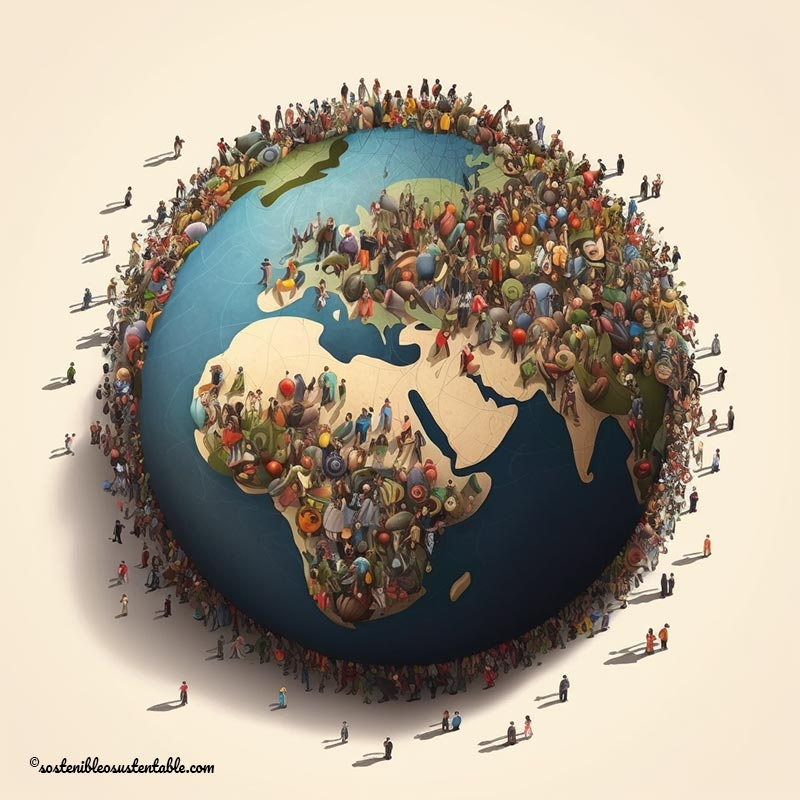
\includegraphics[width=\textwidth]{./media/people.jpg}
	\caption{}
\end{imagen}

En este capítulo se explorarán las tendencias de crecimiento poblacional a nivel mundial y se analizarán las consecuencias sociales y económicas derivadas de este fenómeno. Se utilizarán datos y ejemplos de diferentes regiones del mundo para ilustrar los cambios demográficos recientes.

\section{Tendencias globales}

A lo largo de los siglos, la población mundial ha crecido de manera desigual. La mayoría del crecimiento poblacional se ha concentrado en países en desarrollo, mientras que muchos países desarrollados han experimentado una desaceleración en sus tasas de crecimiento, e incluso, en algunos casos, un decrecimiento.

\subsection{Cifras del crecimiento poblacional}

El cuadro~\ref{cuadro1} muestra la evolución de la población mundial en las últimas décadas, así como las proyecciones futuras para el crecimiento poblacional.

\begin{table}[!ht]
\sf\footnotesize\setlength\tabcolsep{4pt}
\centering
\begin{tabular}{l | cccc}
\toprule
& \textbf{Población & \textbf{Tasa de crecimiento} & \textbf{Esperanza de vida} & \textbf{Población urbana} \\
\textbf{Año} & \textbf{(miles de millones)} & \textbf{(\%)} & \textbf{(años)} & \textbf{(\%)} \\
\midrule
1950 & 2.5 & 1.8 & 48 & 30 \\
\midrule
1980 & 4.4 & 2.1 & 60 & 39 \\
\midrule
2010 & 6.9 & 1.2 & 70 & 51 \\
\midrule
2023 & 8.0 & 1.0 & 72 & 56 \\
\midrule
2050* & 9.7 & 0.8 & 77 & 68\\
\bottomrule
\end{tabular}
\caption{Crecimiento poblacional mundial y proyecciones futuras (*proyecciones).}
\label{cuadro1}
\end{table}

En el cuadro~\ref{cuadro1} se observa cómo la tasa de crecimiento poblacional ha disminuido, mientras que la esperanza de vida y la urbanización han ido en aumento. Las proyecciones indican que la población mundial alcanzará los 9.7 mil millones para 2050, aunque con una tasa de crecimiento más baja que en décadas anteriores.

\section{Factores que afectan el crecimiento poblacional}

El crecimiento de la población está influenciado por varios factores. Entre los más importantes se encuentran las tasas de natalidad, las tasas de mortalidad y las políticas migratorias. A continuación, se presentan algunos de los factores clave que influyen en las dinámicas poblacionales globales.

\begin{table}[!ht]
\sf\footnotesize\setlength\tabcolsep{4pt}
\centering
\begin{tabular}{>{\raggedright\arraybackslash}m{3.4cm} | >{\raggedright\arraybackslash}m{7cm}}
\toprule
\textbf{Factor} & \textbf{Descripción}\\
\midrule
Tasa de natalidad & Cantidad de nacimientos por cada \num{1000} habitantes en un año. \\
\midrule
Tasa de mortalidad & Cantidad de muertes por cada \num{1000} habitantes en un año. \\
\midrule
Esperanza de vida & Número promedio de años que se espera que viva una persona al nacer, influida por factores como la salud y la economía. \\
\midrule
Migración & Movimiento de personas entre regiones, que puede aumentar o disminuir la población de un país o región. \\
\midrule
Políticas gubernamentales & Las políticas de planificación familiar y los incentivos económicos influyen en las tasas de natalidad y mortalidad. \\
\midrule
Condiciones económicas & El crecimiento económico suele estar asociado con una disminución en las tasas de natalidad y mortalidad. \\
\bottomrule
\end{tabular}
\caption{Factores que influyen en el crecimiento poblacional.}
\label{tabla2}
\end{table}

\subsection{Tendencias regionales}

El crecimiento poblacional es especialmente pronunciado en regiones como África subsahariana, donde las tasas de natalidad siguen siendo altas. Sin embargo, en muchas regiones de Europa y Asia Oriental, las tasas de natalidad han caído por debajo del nivel de reemplazo, lo que plantea preocupaciones sobre el envejecimiento de la población y la sostenibilidad de los sistemas de pensiones.

\section{Impacto social y económico}

El crecimiento poblacional tiene efectos significativos en las sociedades y las economías. El rápido aumento de la población puede ejercer presión sobre los recursos naturales, los sistemas de salud, la educación y el empleo. A su vez, un decrecimiento de la población o un envejecimiento significativo puede llevar a la escasez de mano de obra y problemas para mantener el sistema de pensiones.

Los países en desarrollo, con altas tasas de crecimiento, a menudo enfrentan desafíos relacionados con la sostenibilidad de sus recursos. Por otro lado, los países desarrollados que experimentan una disminución en el crecimiento poblacional, deben abordar los problemas del envejecimiento y la escasez de fuerza laboral.

\section{Conclusión}

El crecimiento poblacional es un tema de gran relevancia en la actualidad, con implicaciones profundas para el desarrollo económico y social de las naciones. A medida que la población mundial sigue creciendo, los desafíos de sostenibilidad, planificación urbana y uso de recursos naturales se vuelven más urgentes. Sin embargo, las proyecciones también indican una desaceleración de la tasa de crecimiento, lo que abre una ventana de oportunidad para abordar estos problemas de manera más efectiva.

El análisis de los factores que influyen en el crecimiento poblacional y las variaciones entre regiones nos permite entender mejor las dinámicas demográficas y planificar para un futuro más sostenible.

%	\begin{thebibliography}{9}
%
%		\bibitem{UN2019}
%		United Nations Department of Economic and Social Affairs.
%		\textit{World Population Prospects 2019: Highlights}.
%		United Nations, 2019.
%
%		\bibitem{WorldBank2021}
%		World Bank.
%		\textit{World Development Indicators: Population Dynamics}.
%		World Bank, 2021.
%
%	\end{thebibliography}

